
% -- --------------------------------------------------------------------------------------------------- -- %
% -- posteR-knitR: Templates for LaTeX (Beamer) and R Programming (knitR) for research posters           -- %
% -- --------------------------------------------------------------------------------------------------- -- %
% -- Description: Beamer poster LaTeX format and knitR R package bindings for research posters           -- %
% -- poster.rnw: File with LaTeX and R codes                                                             -- %
% -- Author: IFFranciscoME - if.francisco.me@gmail.com                                                   -- %
% -- license: MIT License                                                                                -- %
% -- Repository: https://github.com/IFFranciscoME/posteR-knitR                                           -- %
% -- --------------------------------------------------------------------------------------------------- -- %

\documentclass{postertheme}\usepackage[]{graphicx}\usepackage[]{color}
% maxwidth is the original width if it is less than linewidth
% otherwise use linewidth (to make sure the graphics do not exceed the margin)
\makeatletter
\def\maxwidth{ %
  \ifdim\Gin@nat@width>\linewidth
    \linewidth
  \else
    \Gin@nat@width
  \fi
}
\makeatother

\definecolor{fgcolor}{rgb}{0.345, 0.345, 0.345}
\newcommand{\hlnum}[1]{\textcolor[rgb]{0.686,0.059,0.569}{#1}}%
\newcommand{\hlstr}[1]{\textcolor[rgb]{0.192,0.494,0.8}{#1}}%
\newcommand{\hlcom}[1]{\textcolor[rgb]{0.678,0.584,0.686}{\textit{#1}}}%
\newcommand{\hlopt}[1]{\textcolor[rgb]{0,0,0}{#1}}%
\newcommand{\hlstd}[1]{\textcolor[rgb]{0.345,0.345,0.345}{#1}}%
\newcommand{\hlkwa}[1]{\textcolor[rgb]{0.161,0.373,0.58}{\textbf{#1}}}%
\newcommand{\hlkwb}[1]{\textcolor[rgb]{0.69,0.353,0.396}{#1}}%
\newcommand{\hlkwc}[1]{\textcolor[rgb]{0.333,0.667,0.333}{#1}}%
\newcommand{\hlkwd}[1]{\textcolor[rgb]{0.737,0.353,0.396}{\textbf{#1}}}%
\let\hlipl\hlkwb

\usepackage{framed}
\makeatletter
\newenvironment{kframe}{%
 \def\at@end@of@kframe{}%
 \ifinner\ifhmode%
  \def\at@end@of@kframe{\end{minipage}}%
  \begin{minipage}{\columnwidth}%
 \fi\fi%
 \def\FrameCommand##1{\hskip\@totalleftmargin \hskip-\fboxsep
 \colorbox{shadecolor}{##1}\hskip-\fboxsep
     % There is no \\@totalrightmargin, so:
     \hskip-\linewidth \hskip-\@totalleftmargin \hskip\columnwidth}%
 \MakeFramed {\advance\hsize-\width
   \@totalleftmargin\z@ \linewidth\hsize
   \@setminipage}}%
 {\par\unskip\endMakeFramed%
 \at@end@of@kframe}
\makeatother

\definecolor{shadecolor}{rgb}{.97, .97, .97}
\definecolor{messagecolor}{rgb}{0, 0, 0}
\definecolor{warningcolor}{rgb}{1, 0, 1}
\definecolor{errorcolor}{rgb}{1, 0, 0}
\newenvironment{knitrout}{}{} % an empty environment to be redefined in TeX

\usepackage{alltt}

\usepackage{lipsum}                                % Package for dummy text
\usepackage[absolute, overlay]{textpos}            % Figure placement
\usepackage{graphicx}
\usepackage{float}

\setlength{\TPHorizModule}{\paperwidth}
\setlength{\TPVertModule}{\paperheight}

\usepackage{pgfplots}
\pgfplotsset{compat=1.14,           % <-- added
            width=\columnwidth,     % <-- added
            height=0.75\columnwidth % <-- added, with this the image is in aspect 4:3
            }

\title{Here you can put an awesome and representative title}

\vskip4cm

\author {
  First author name \inst{1}
  \and
  Second author name \inst{2}
  }

\institute {
  \inst{1} Academic institute
  \and
  \inst{2} Industry research center
  }

% -- ------------------------------------------------------------------------- CODE 1: SOME CALCULATIONS -- %
% -- ------------------------------------------------------------------------- ------------------------- -- %



\IfFileExists{upquote.sty}{\usepackage{upquote}}{}
\begin{document}

\begin{frame}

% -- -------------------------------------------------------------------------------------- ----------- -- %
% -- -------------------------------------------------------------------------------------- ----------- -- %

\begin{columns}[onlytextwidth]
  
  \begin{column}{1 \textwidth - 0.01 \textwidth}
    \begin{block}{Block Title}
    
      \lipsum[1]
      
       
      
    \end{block}
  \end{column}
\end{columns}

% -- -------------------------------------------------------------------------------------- ----------- -- %
% -- -------------------------------------------------------------------------------------- ----------- -- %

\begin{columns}[onlytextwidth]
  
  \begin{column}{.75 \textwidth - 0.01 \textwidth}
    \begin{block}{Block Title}
      One core component of the predictive mopdeling prrocess is to add the regularization
      criteria \textit{elasticnet}, for the Cost Function that is being minimized in the
      weight updating process:

      \begin{equation}
          J(w) =  J(w) + C \frac{\lambda}{m} \sum_{j=1}^n \left \lVert w_j \right\rVert_1 + (1 - C) 
          \frac{\lambda}{2m} \sum_{j=1}^n \left \lVert w_j \right\rVert_2^2
      \end{equation}

      \footnotesize
      \noindent
      $L_{1}$: Also known as $Lasso$  \\
      $L_{2}$: Also known as $Ridge$ \\
      $C$: A coefficient to regulate the effect between $L_{1}$ and $L_{2}$

    \end{block}
  \end{column}

  \begin{column}{.25 \textwidth - 0.01 \textwidth}
    \begin{block}{Block Title}
      
          \begin{figure}
            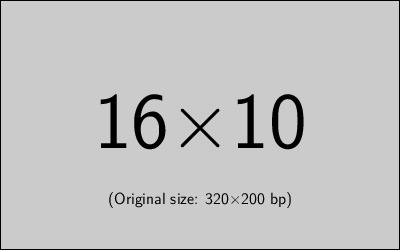
\includegraphics[scale=1]{figures/example-image-16x10.jpg}
            \caption{This is a caption}
          \end{figure}

    \end{block}
  \end{column}

\end{columns}

% -- -------------------------------------------------------------------------------------- ----------- -- %
% -- -------------------------------------------------------------------------------------- ----------- -- %

\begin{columns}[onlytextwidth]
  
  \begin{column}{.5 \textwidth - 0.01 \textwidth}
    \begin{block}{Block Title}
      \begin{minipage}{\linewidth}
        \begin{minipage}{0.5 \linewidth}
          \begin{figure}
            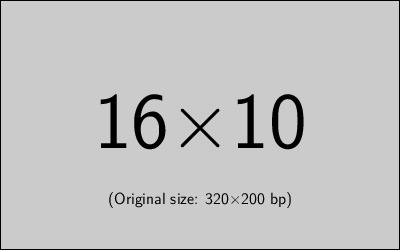
\includegraphics[scale=1]{figures/example-image-16x10.jpg}
            \caption{This is a caption}
          \end{figure}
        \end{minipage}
        \hfill
        \begin{minipage}{0.5 \linewidth}
          \begin{figure}
            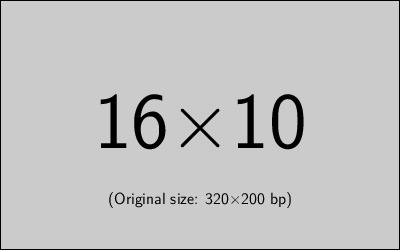
\includegraphics[scale=1]{figures/example-image-16x10.jpg}
            \caption{This is a caption}
          \end{figure}
        \end{minipage}
      \end{minipage}
    \end{block}
  \end{column}

  \begin{column}{.5 \textwidth - 0.01 \textwidth}
    \begin{block}{Block Title}
      \lipsum[2]
    \end{block}
  \end{column}
  
\end{columns}

% -- -------------------------------------------------------------------------------------- ----------- -- %
% -- -------------------------------------------------------------------------------------- ----------- -- %

\begin{columns}[onlytextwidth]
  
  \begin{column}{.25 \textwidth - 0.01 \textwidth}
    \begin{block}{Block Title}
      \lipsum[4]
    \end{block}
  \end{column}

  \begin{column}{.25 \textwidth - 0.01 \textwidth}
    \begin{block}{Block Title}
      \lipsum[4]
    \end{block}
  \end{column}

  \begin{column}{.25 \textwidth - 0.01 \textwidth}
    \begin{block}{Block Title}
      
      \begin{table}
        \centering
        \begin{tabular}{|l|l|l|}
        \hline
        \multicolumn{1}{|c|}{Metric} & \multicolumn{1}{c|}{Value 1} & \multicolumn{1}{c|}{Value 2} \\ \hline
        acc-train        & 0.9155 & 0.8311 \\ \hline
        acc-val          & 0.8245 & 0.7368 \\ \hline
        acc-mean         & 0.8700 & 0.7839 \\ \hline
        acc-diff         & 0.0909 & 0.0942 \\ \hline
        acc-weighted     & 0.4486 & 0.4061 \\ \hline
        acc-inv-weighted & 0.4213 & 0.3778 \\ \hline
        auc-train        & 0.9924 & 0.9300 \\ \hline
        auc-val          & 0.8401 & 0.8017 \\ \hline
        \end{tabular}
        
        \vskip0.35in
        \caption{This is caption}
        \label{tab:my-table}
        \end{table}
      
    \end{block}
  \end{column}

  \begin{column}{.25 \textwidth - 0.01 \textwidth}
    \begin{block}{Block Title}
      \lipsum[4]
    \end{block}
  \end{column}

\end{columns}

% -- -------------------------------------------------------------------------------------- ----------- -- %
% -- -------------------------------------------------------------------------------------- ----------- -- %

\begin{columns}[onlytextwidth]
  
  \begin{column}{.25 \textwidth - 0.01 \textwidth}
    \begin{block}{Block Title}
    \begin{figure}
    
      \begin{minipage}{\linewidth}
        \begin{minipage}{0.49 \linewidth}
          \begin{figure}
            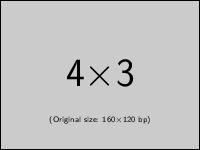
\includegraphics[scale=1]{figures/example-image-4x3.jpg}
          \end{figure}
        \end{minipage}
        \hfill
        \begin{minipage}{0.49 \linewidth}
          \begin{figure}
            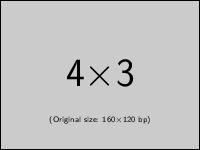
\includegraphics[scale=1]{figures/example-image-4x3.jpg}
          \end{figure}
        \end{minipage}
      \end{minipage}
      \vfill
      \begin{minipage}{\linewidth}
        \begin{minipage}{0.49 \linewidth}
          \begin{figure}
            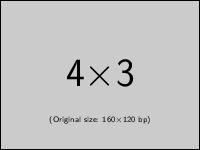
\includegraphics[scale=1]{figures/example-image-4x3.jpg}
          \end{figure}
        \end{minipage}
        \hfill
        \begin{minipage}{0.49 \linewidth}
          \begin{figure}
            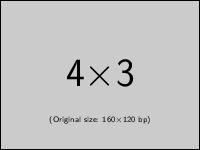
\includegraphics[scale=1]{figures/example-image-4x3.jpg}
          \end{figure}
        \end{minipage}
      \end{minipage}
      
    \vskip0.25in
    \caption{This is a caption}
    \end{figure}
    \end{block}
  \end{column}

  \begin{column}{.75 \textwidth - 0.01 \textwidth}
    \begin{block}{Block Title}
      \lipsum[4-5]
    \end{block}
  \end{column}

\end{columns}

% -- -------------------------------------------------------------------------------------- ----------- -- %
% -- -------------------------------------------------------------------------------------- ----------- -- %

\begin{columns}[onlytextwidth]
  
  \begin{column}{.5 \textwidth - 0.01 \textwidth}
    \begin{block}{Block Title}
    \begin{figure}

        \begin{minipage}{0.2 \linewidth}
          \begin{figure}
            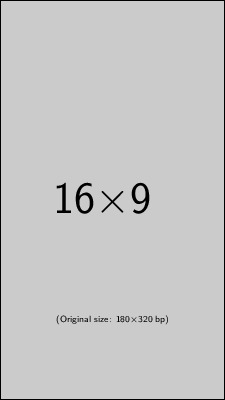
\includegraphics[scale=1]{figures/example-image-9x16.jpg}
          \end{figure}
        \end{minipage}
        \hskip0.45in
        \begin{minipage}{0.2 \linewidth}
          \begin{figure}
            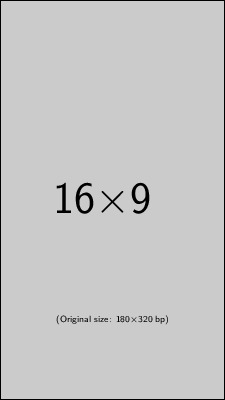
\includegraphics[scale=1]{figures/example-image-9x16.jpg}
          \end{figure}
        \end{minipage}
        \hskip0.45in
        \begin{minipage}{0.2 \linewidth}
          \begin{figure}
            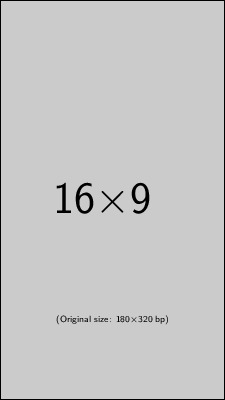
\includegraphics[scale=1]{figures/example-image-9x16.jpg}
          \end{figure}
        \end{minipage}
        \hskip0.45in
        \begin{minipage}{0.2 \linewidth}
          \begin{figure}
            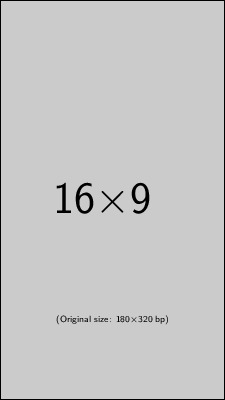
\includegraphics[scale=1]{figures/example-image-9x16.jpg}
          \end{figure}
        \end{minipage}

    \vskip0.25in
    \caption{This is a caption}      
  \end{figure}
    
    \end{block}
  \end{column}
  
  \begin{column}{.5 \textwidth - 0.01 \textwidth}
    \begin{block}{Block Title}
    
    \lipsum[7]
    
    \end{block}
  \end{column}
\end{columns}


% -- -------------------------------------------------------------------------------------- ----------- -- %

\end{frame}
\end{document}
